% Befehl \fibelvorstellung: Erstellt die Vorstellung eines FSlers mit Bild
%	Parameter #1: Bild (wrapfigure)
%	Parameter #2: Text
\newcommand{\fibelvorstellung}[2]{%
	\begin{minipage}{\columnwidth}
		% Kein Abstand vor bzw. nach Bildern bei wrapfigure
		\setlength{\intextsep}{0cm}
		% geringfügiger Abstand zwischen Paragraphen
		\setlength{\parskip}{0.5ex}
		#1
		#2
		\vspace{0.5ex}
	\end{minipage}
	
	\vspace{5ex plus 2ex minus 1ex}
}
\newlength{\fibelstdlen}
\setlength{\fibelstdlen}{3.7cm}

\section{Der Fachschaftsrat~(FSR) Physik stellt sich vor}
\begin{multicols*}{2}

\fibelvorstellung{
	\begin{wrapfigure}{l}{0cm}
		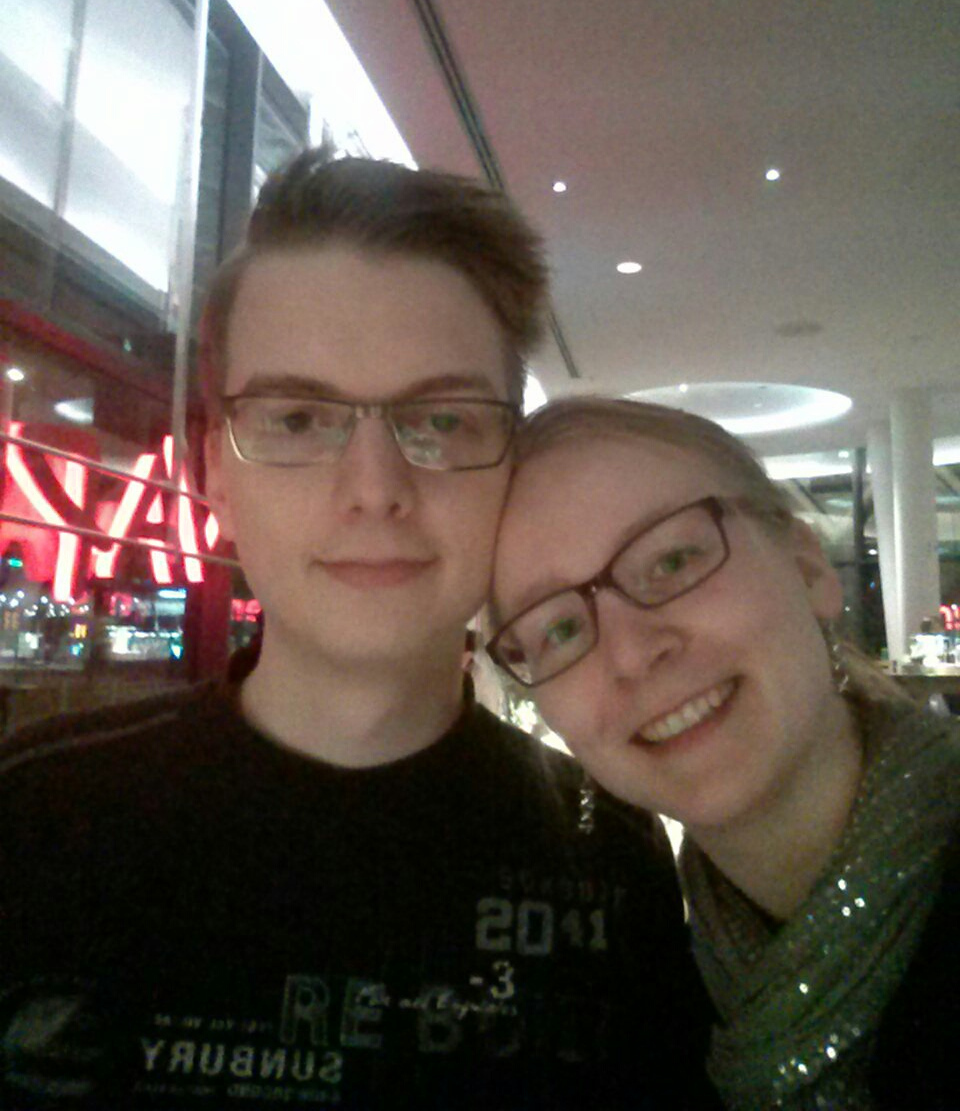
\includegraphics[width=5.1cm]{res/vorstellungsfotos/simon_may_alexandra_everwand_edited_cropped}
	\end{wrapfigure}
}
{% LaTeX-Warnung deaktivieren
%\hbadness=10000

Hey,
wir sind Alex (rechts) und Simon (links), das "Fachschaftspärchen".
Da man uns eigentlich nie getrennt antreffen kann, stellen wir uns hier 
gemeinsam vor – das kommt der Realität näher ;-)
Wir sind im Master und waren gemeinsam ein Jahr in Schweden.
Ich (Simon) kann euch bei technischen und Computer-bezogenen Fragen weiterhelfen; ich (Alex) organisiere z\,.B.\ die O-Woche, den Buchmarkt und bei den Spieleabenden helfe ich auch immer mit.
Fragt aber auch sonst ruhig nach, wenn ihr Hilfe braucht :-)
}
	
\fibelvorstellung{
	\begin{wrapfigure}{r}{0cm}
		\includegraphics[width=\fibelstdlen]{res/vorstellungsfotos/benedikt_bieringer}
	\end{wrapfigure}
}
{Hallo zusammen! Mein Name ist Benedikt. In der Fachschaft bin ich für so ziemlich alles verantwortlich, was mit Computergrafik/Design zu tun hat. Programmieren und Schwimmen sind nur zwei meiner weiteren Freizeitbeschäftigungen. In meinen jetzt 6~Semestern Fachschafts- und Studienerfahrung kann ich euch aber auch bei einer ganzen Reihe weiterer Fragen weiterhelfen.}

\fibelvorstellung{
	\begin{wrapfigure}{l}{0cm}
		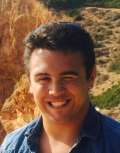
\includegraphics[width=\fibelstdlen]{res/vorstellungsfotos/fernando_romahn.png}
	\end{wrapfigure}
}
{Hey Leute, ich bin Fernando (der Name ist ostfriesisch auszusprechen). Ich studiere jetzt seit 6 Semestern Physik und bin aktueller Vorsitzender der Fachschaft. Zumeist bin ich ein ruhiger und gut gelaunter Typ (außer bei Mario Kart, da kenn ich keine Freunde). Bei Fragen, Anregungen oder Lobeshymnen auf mich habe ich immer ein offenes Ohr für euch :\^{})}

	
\fibelvorstellung{
	\begin{wrapfigure}{r}{0cm}
		\includegraphics[width=1.14\fibelstdlen]{res/vorstellungsfotos/benedikt_stauff}
	\end{wrapfigure}
}
{Hi, ich bin Benedikt Stauff und studiere momentan im 3.~Semester Physik als 1-Fach-Bachelor. 
Ich bin seit meinem ersten Semester in der Fachschaft. Falls ihr irgendwelche Fragen habt wendet euch ruhig an mich.}

\fibelvorstellung{
	\begin{wrapfigure}{l}{0cm}
		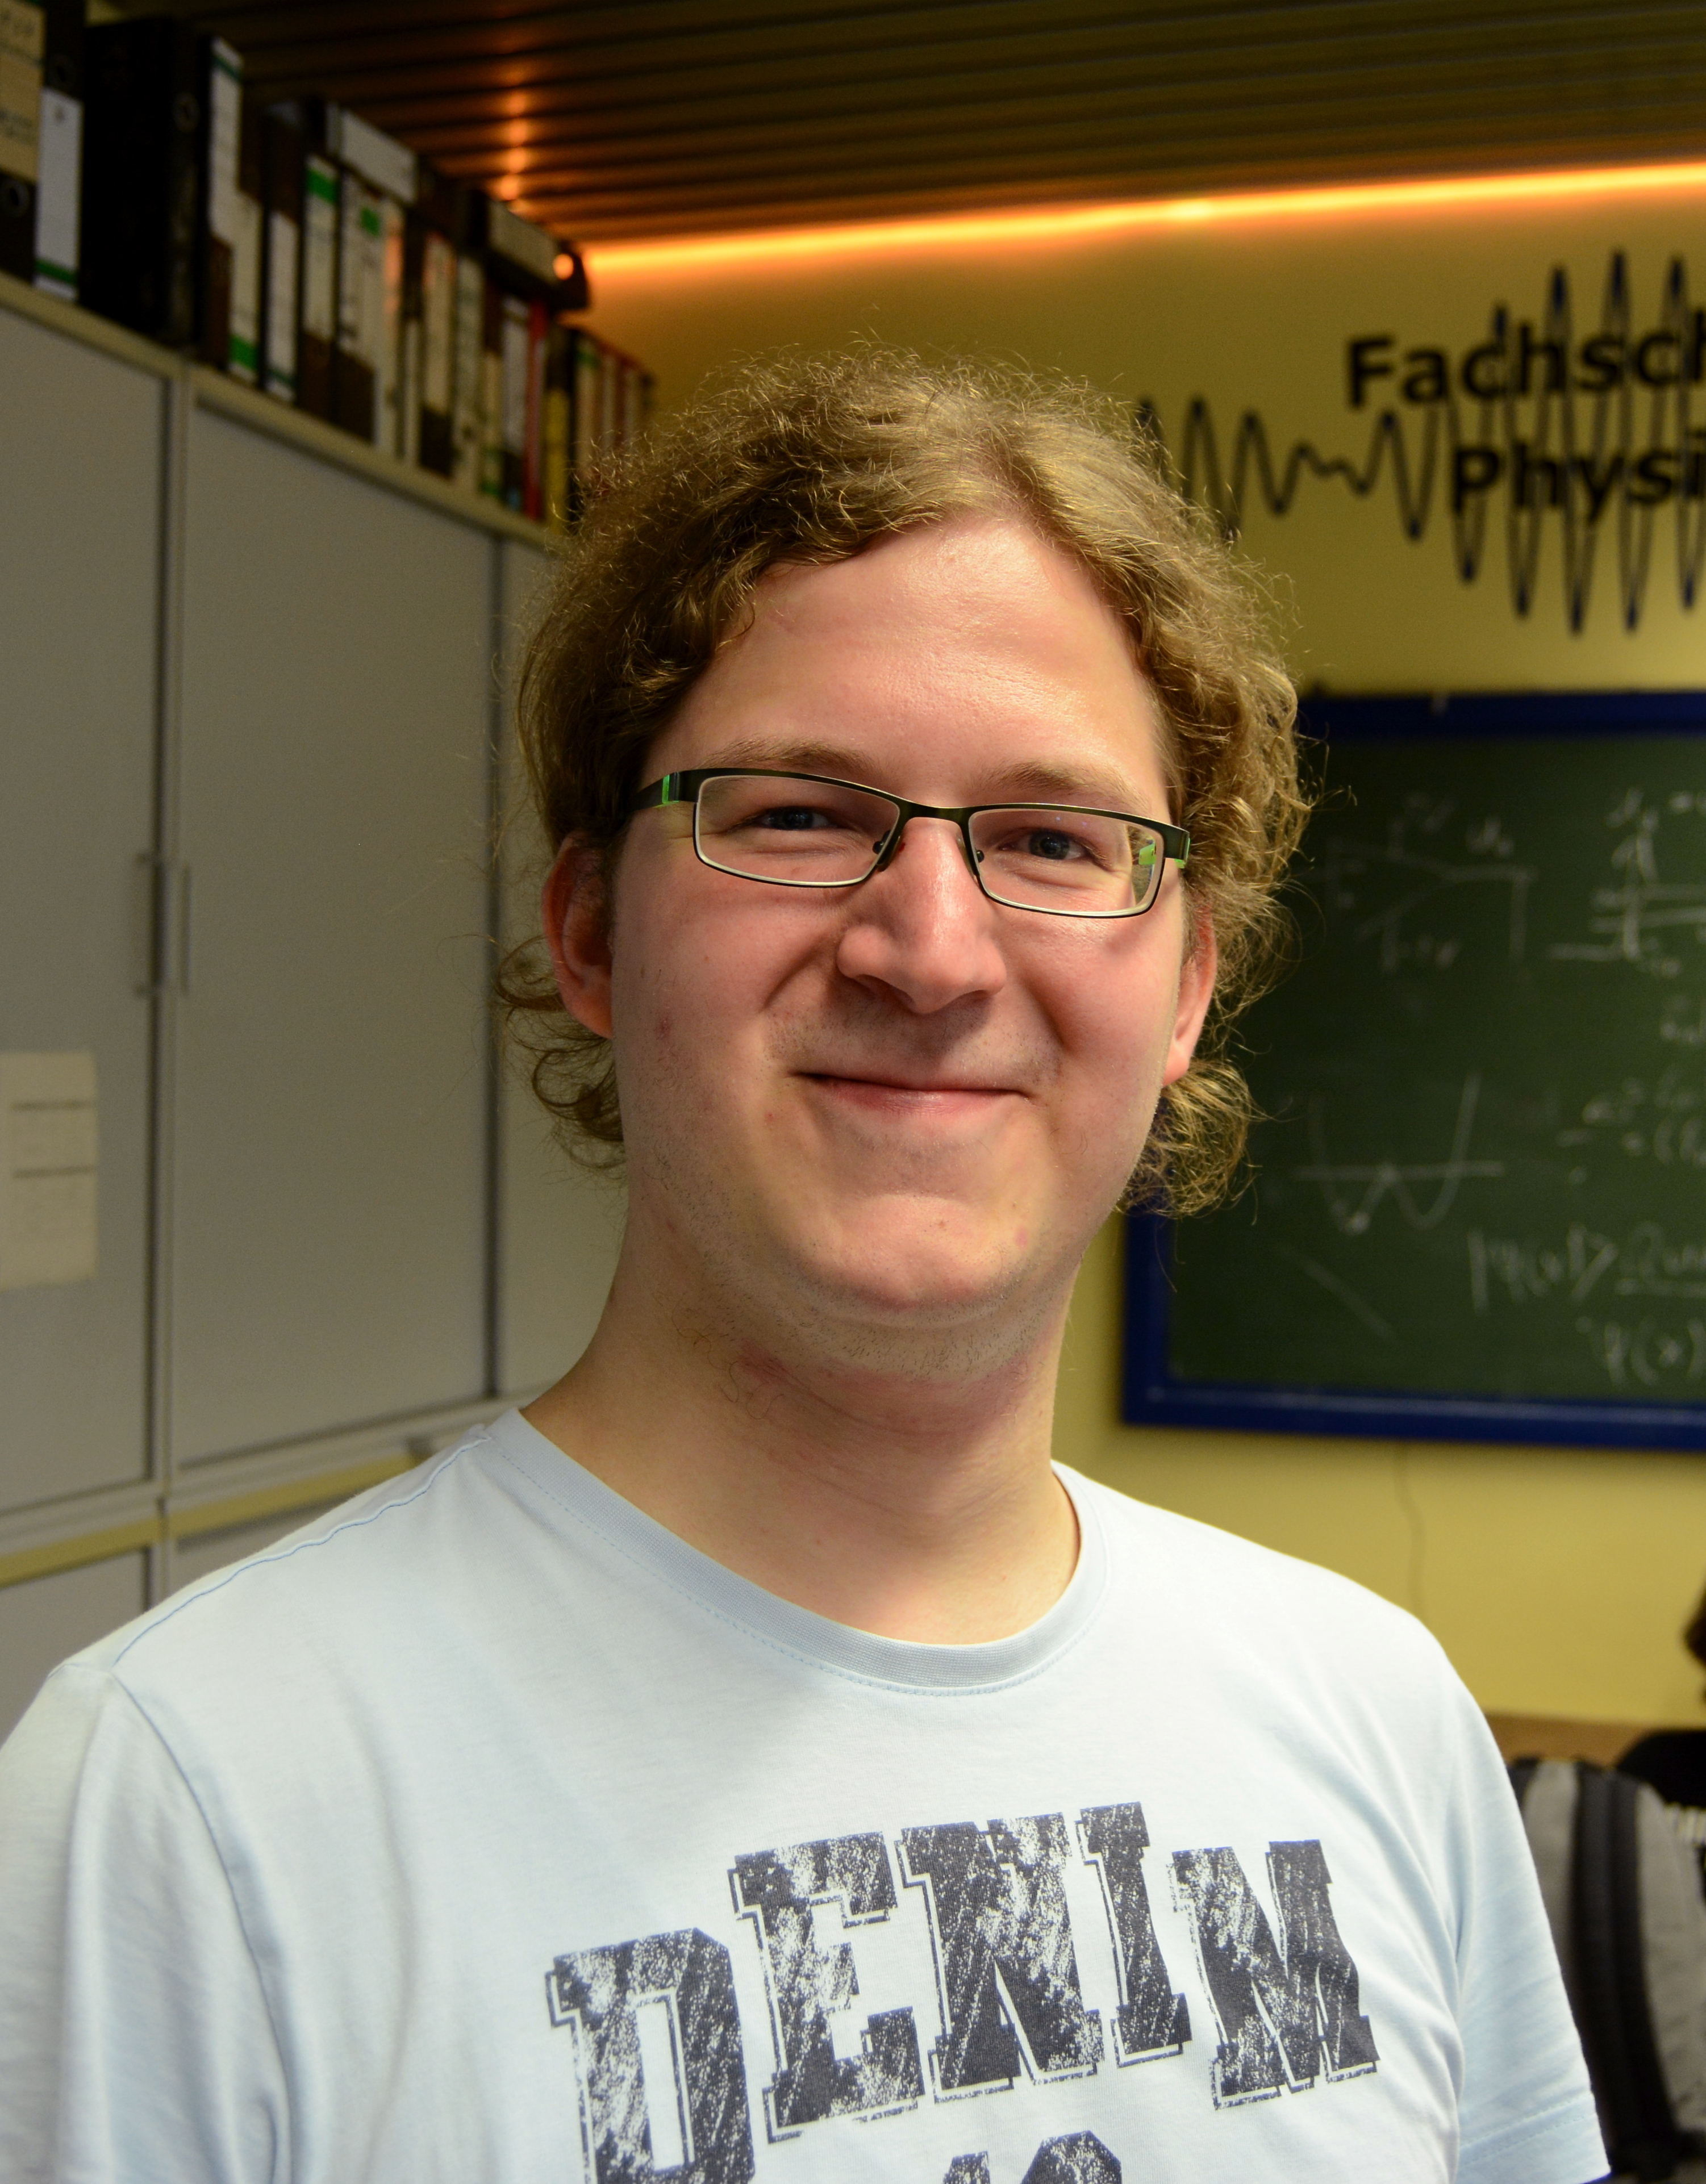
\includegraphics[width=\fibelstdlen]{res/vorstellungsfotos/bernd_hofschroeer_cropped}
	\end{wrapfigure}
}
{Ich bin Bernd, bin im höheren Semester und studiere den Master of Education Physik-Chemie, werde also Lehrer. Ich bin seit meinem 3.\ Semester in der Fachschaft und hoffe, euch mal auf den Spieleabenden zu treffen!
\vspace{2\baselineskip}
}
\fibelvorstellung{
	\begin{wrapfigure}{r}{0cm}
		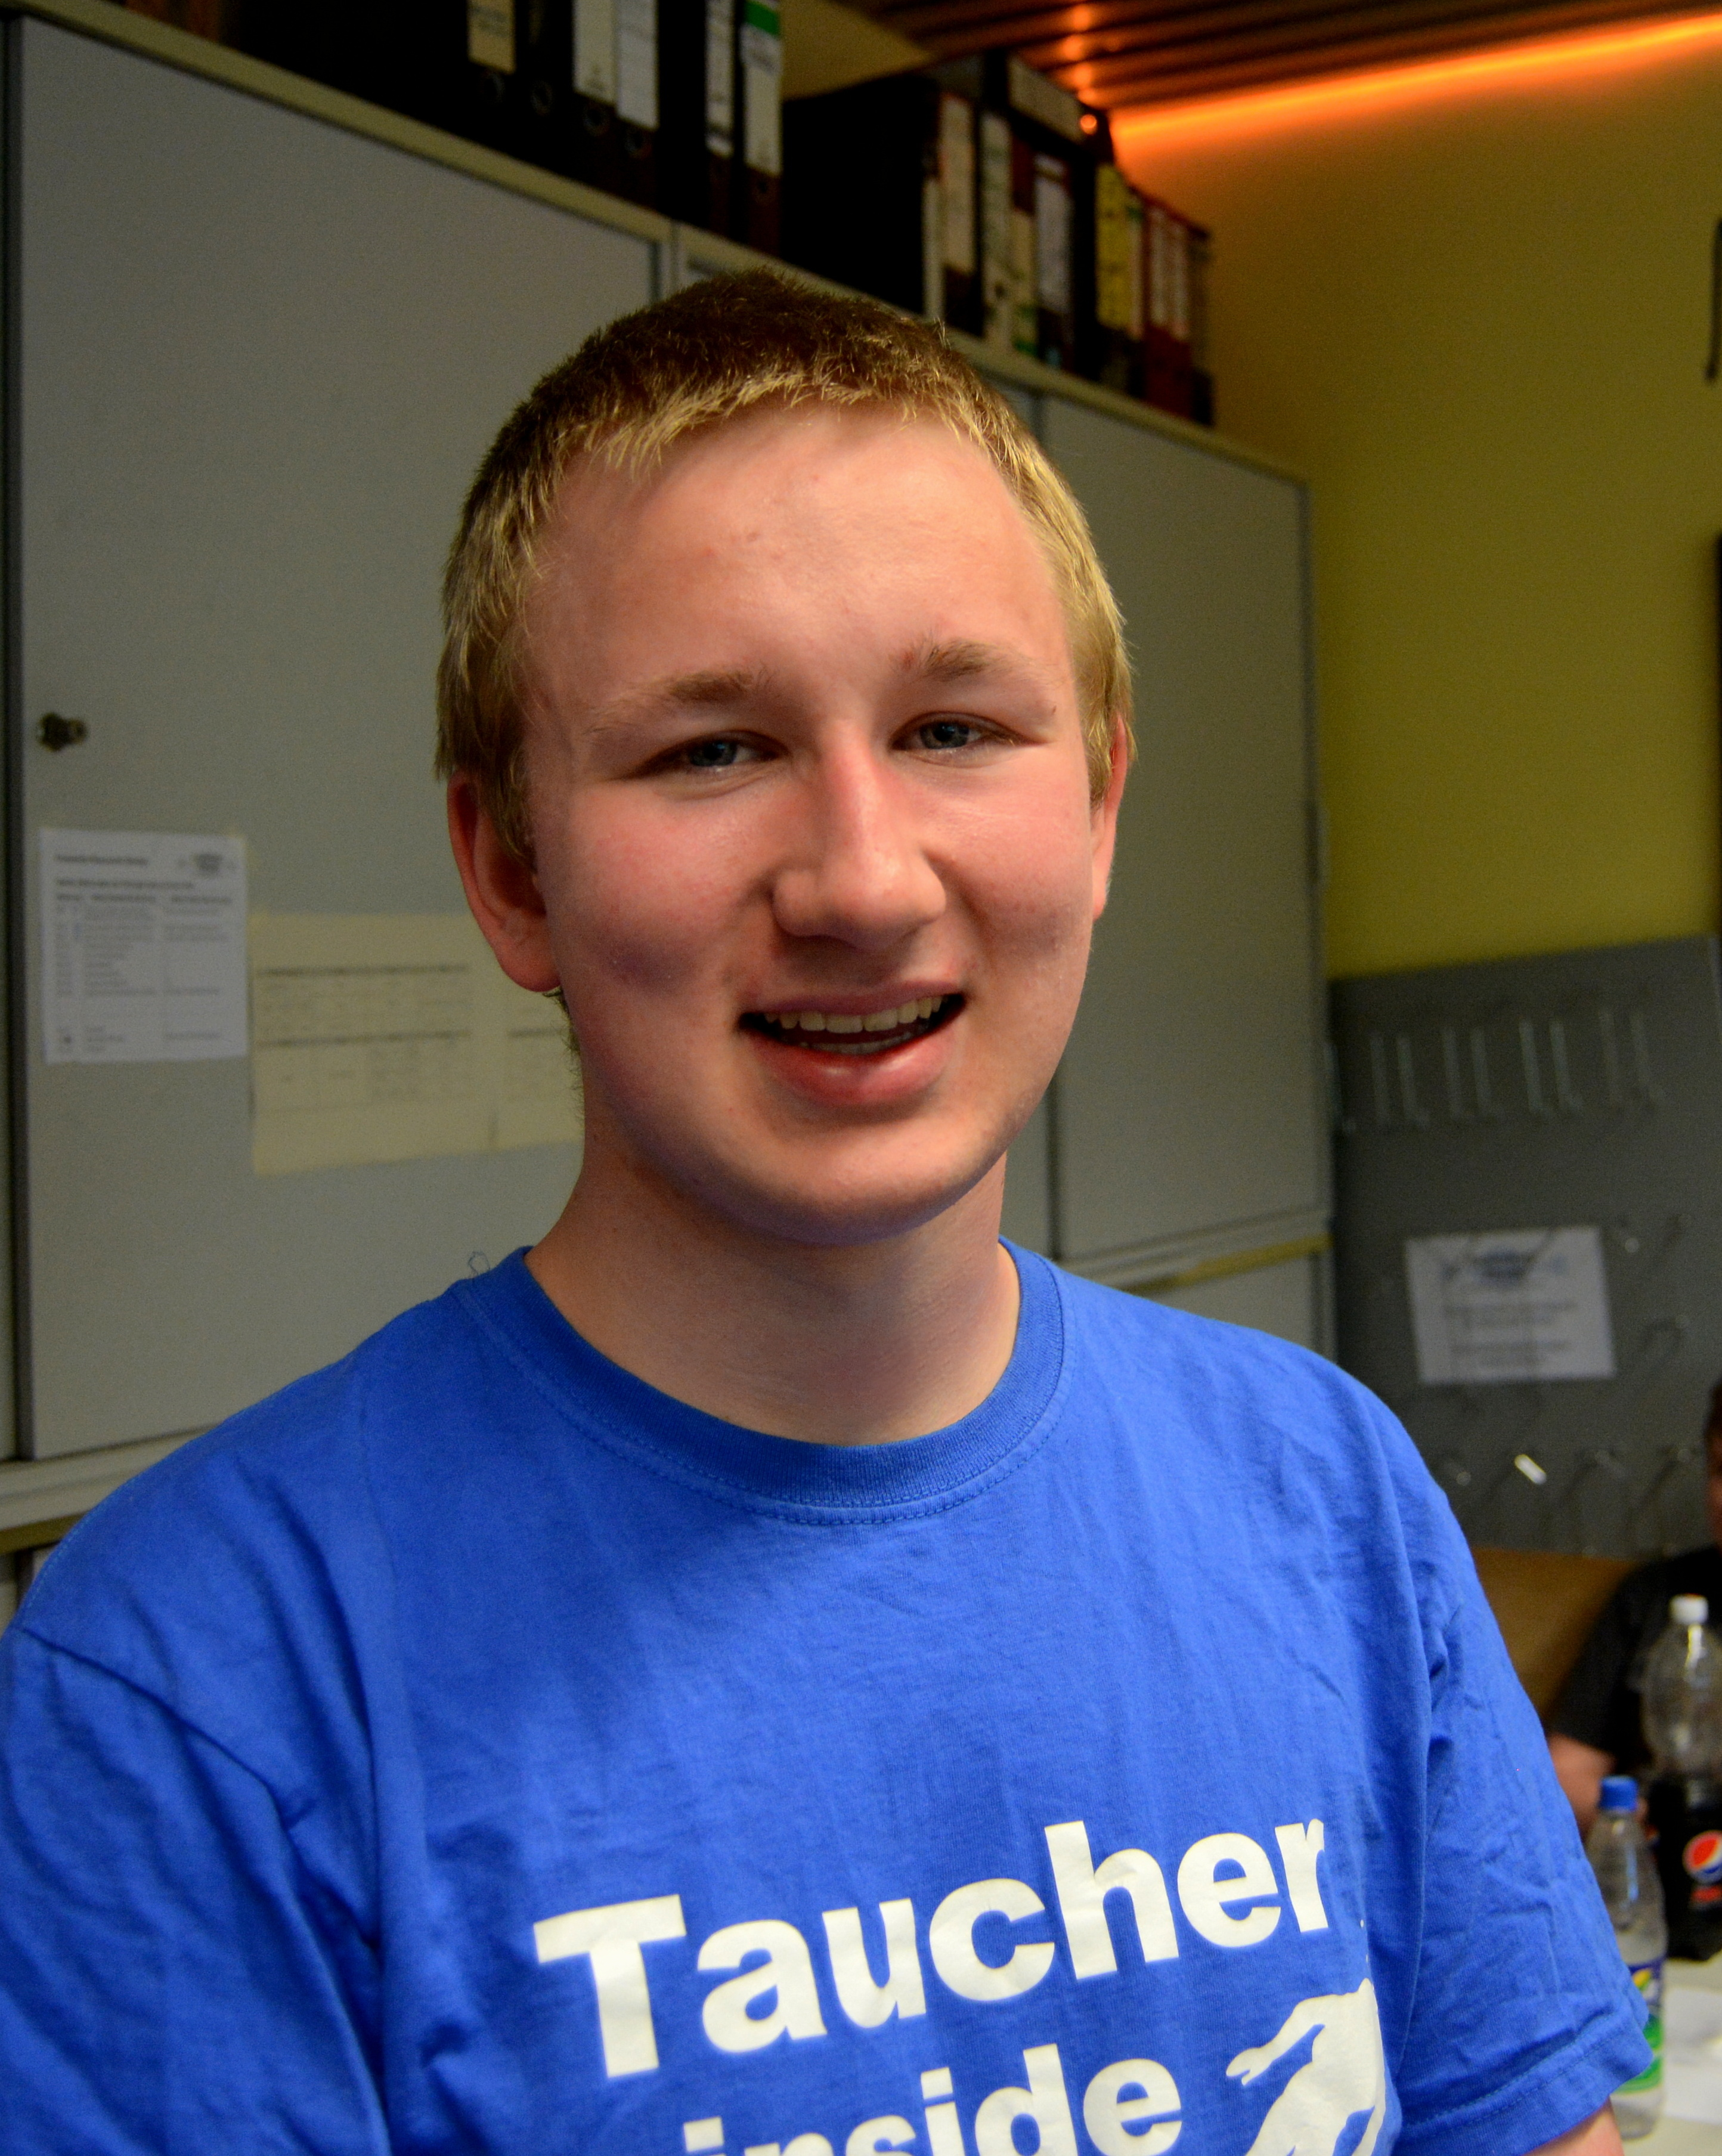
\includegraphics[width=\fibelstdlen]{res/vorstellungsfotos/hauke_hawighorst_cropped}
	\end{wrapfigure}
}
{Moin, ich bin Hauke und im dritten Semester. Vor allem kümmere ich mich um die Evaluation der Lehrveranstaltungen. An euch ein herzliches Willkomen in Münster!
\vspace{2\baselineskip}}

\fibelvorstellung{
	\begin{wrapfigure}{l}{0cm}
		\includegraphics[width=\fibelstdlen]{res/vorstellungsfotos/lutz_althueser_cropped.jpg}
	\end{wrapfigure}
}
{Haii! Ich bin Lutz und mittlerweile am Ende des Masterstudiums angelangt. Der Fachschaft bin ich vor unvorstellbaren 5 Jahren in meinem eigenen ersten Semester beigetreten. In der Fachschaft werdet Ihr mich nur noch selten antreffen, dafür bin ich aber jederzeit in meinem Büro und kann bei jeder Angelegenheit helfen. Neben vielen kleinen Aufgaben kümmere ich mich hauptsächlich nur noch darum das meine ehemaligen Aufgabenbereiche in der Fachschaft auch in Zukunft übernommen werden.

Also bis (vielleicht) bald! }

\fibelvorstellung{
	\begin{wrapfigure}{r}{0cm}
		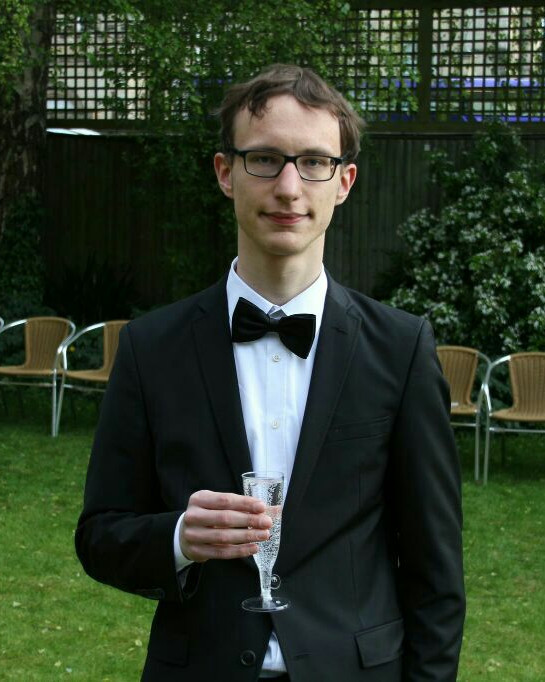
\includegraphics[width=\fibelstdlen]{res/vorstellungsfotos/michael_te_vrugt_cropped}
	\end{wrapfigure}
}
{Hi, ich bin Michael, studiere im 7. Semester Physik und Philosophie und bin kürzlich von einem Jahr in Oxford zurückgekehrt. Bei Fragen zur Philosophie, einem Doppelstudium, Stipendien oder irgendetwas anderem stehe ich euch jederzeit zur Verfügung. Ansonsten wünsche ich euch viel Spaß in der O-Woche und im Studium!}

\fibelvorstellung{
	\begin{wrapfigure}{l}{0cm}
		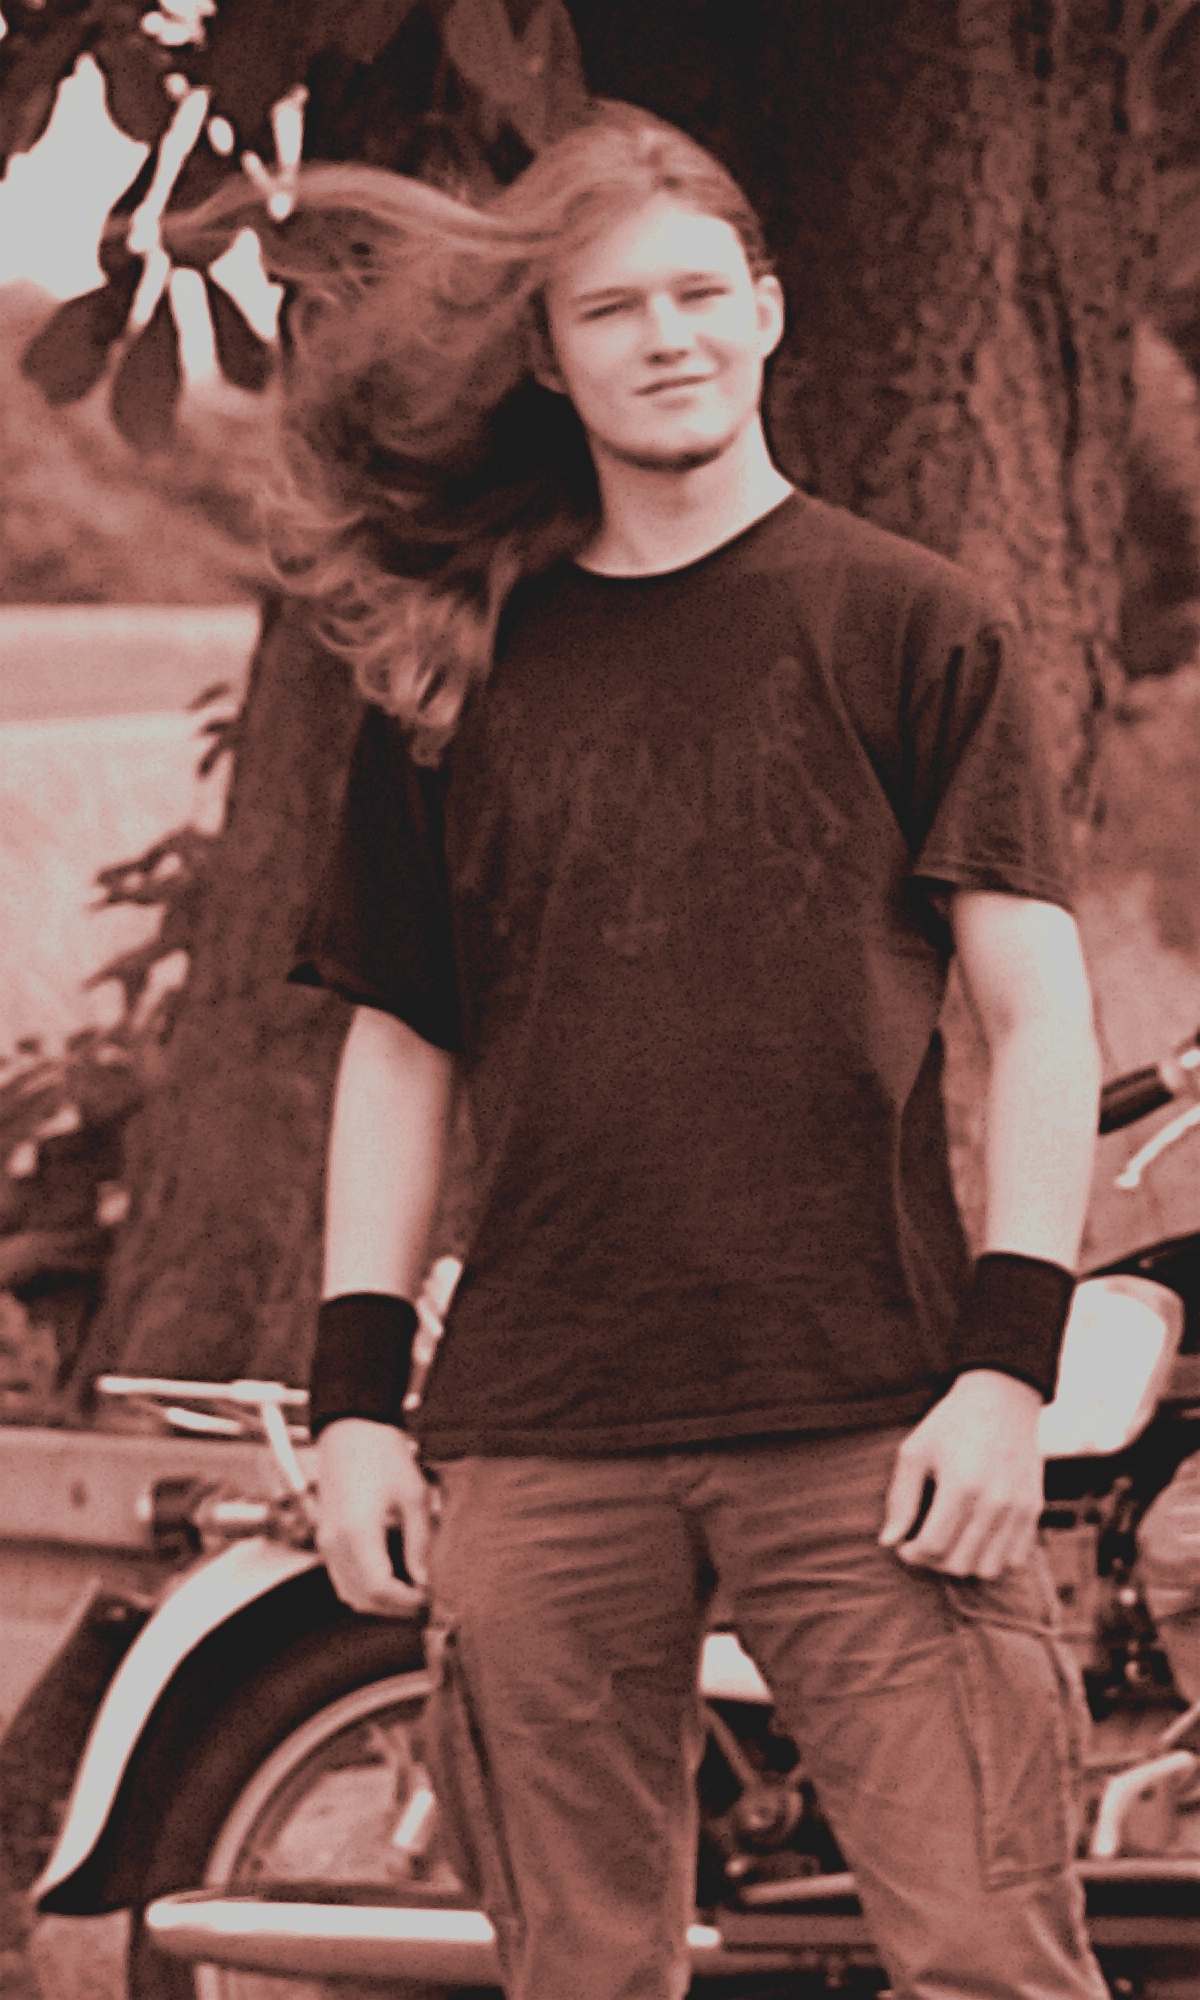
\includegraphics[width=\fibelstdlen]{res/vorstellungsfotos/jan_honermann}
	\end{wrapfigure}
}
{Hi, ich bin Jan und sitze gerade an meiner Masterarbeit. Falls ihr Fragen habt, könnt ihr euch gerne an mich wenden, ich bin meistens netter, als ich aussehe ;)
\vspace{\baselineskip}
}

\fibelvorstellung{
	\begin{wrapfigure}{r}{0cm}
		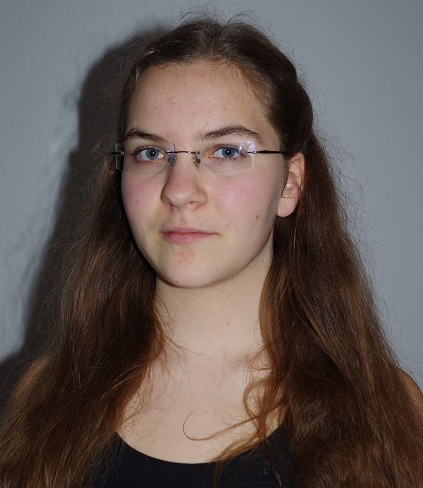
\includegraphics[width=\fibelstdlen]{res/vorstellungsfotos/andrea_garner_cropped}
	\end{wrapfigure}
}
{Hallo, ich bin Andrea und studiere seit dem WS 2016 Physik und Musik (2FB). Sollten ihr Fragen in Sachen Lehramt haben könnt ihr mich gerne ansprechen :)
\vspace{\baselineskip}
}


\fibelvorstellung{
	\begin{wrapfigure}{l}{0cm}
		
\includegraphics[width=\fibelstdlen]{res/vorstellungsfotos/jan_kirchner}
	\end{wrapfigure}
}
{Hey liebe Erstis, ich bin Jan und studiere hier nun bereits seit 2 Semestern Physik. Im ersten Semester habe ich mich schon recht früh in der Fachschaft wiedergefunden und bin sehr gerne bereit euch als ein noch recht neuer Student ein paar Starttipps oder Antworten zu dem ersten Jahr Physik mit auf den Weg zu geben. Sich in die Uni- und Fachschaftsarbeit zu integrieren und sich auch außerhalb des Studiums zu engagieren kann ich euch zusätzlich wärmstens empfehlen.

Nun jedoch viel Spaß in der O-Woche (und viel Erfolg danach)!
}

\fibelvorstellung{
	\begin{wrapfigure}{r}{0cm}
		\includegraphics[width=\fibelstdlen]{res/vorstellungsfotos/johanna_jakob}
	\end{wrapfigure}
}
{Moin! Ich bin Johanna und fange in diesem Semester mit dem letzten Bachelorjahr an. In der Fachschaft bin ich von Anfang an dabei und momentan als Finanzer tätig.
\vspace{2\baselineskip}}

\fibelvorstellung{
	\begin{wrapfigure}{l}{0cm}
		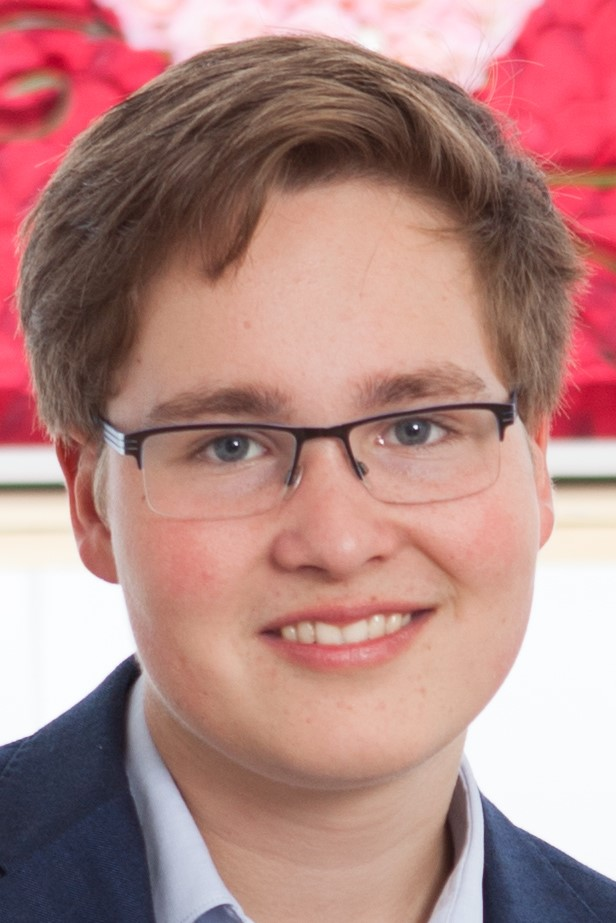
\includegraphics[width=.95\fibelstdlen]{res/vorstellungsfotos/jonas_luebken}
	\end{wrapfigure}
}
{Moin zusammen,
mein Name ist Jonas, ich studiere Physik und Mathematik jeweils im 1-Fach-Bachelor im dritten Semester.
Ich bringe mich sehr gerne in Gremien ein, um die Interessen der Studierenden dort zu vertreten, bin aber auch sonst bei allem, was die Fachschaft tut dabei.
In meiner Freizeit spiele ich ansonstern noch Rollstuhlbasketball.
Ihr könnt gerne jederzeit mit Fragen zum Studium allgemein oder insbesondere zum Nebenfach Mathematik stellen :)
\vspace{\baselineskip}}

\fibelvorstellung{
	\begin{wrapfigure}{r}{0cm}
		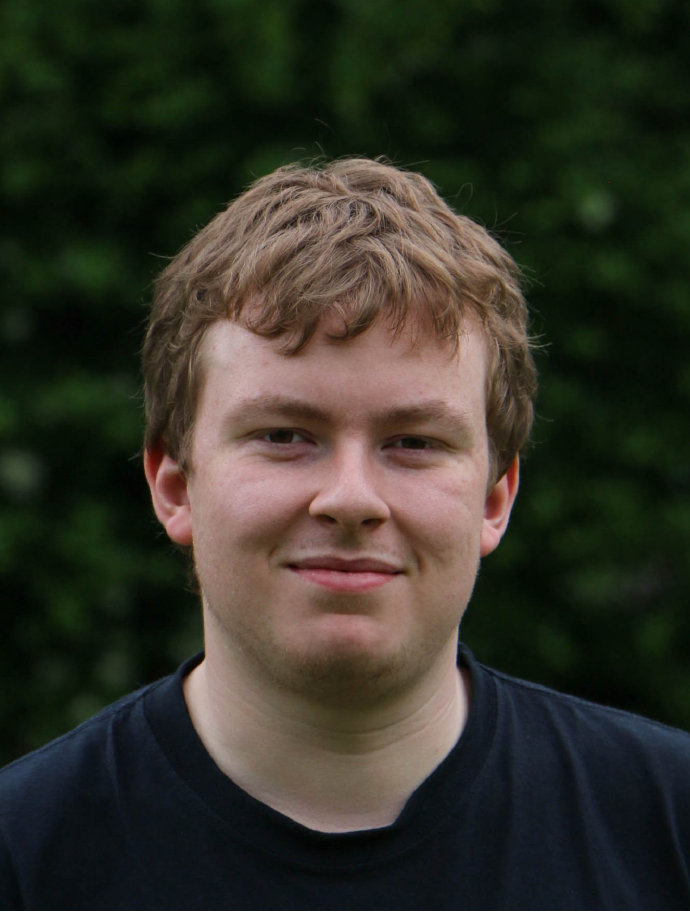
\includegraphics[width=\fibelstdlen]{res/vorstellungsfotos/maik_stappers}
	\end{wrapfigure}
}
{Heyho. Ich bin Maik und mittlerweile Promotionsstudent. Nach nun mehr 5 Jahren in diesem Irrenhaus kann ich euch alle Fragen rund ums Studium und die Uni beantworten. Innerhalb der Fachschaft ist mein Steckenpferd die Hochschulpolitik.}

\fibelvorstellung{
	\begin{wrapfigure}{l}{0cm}
		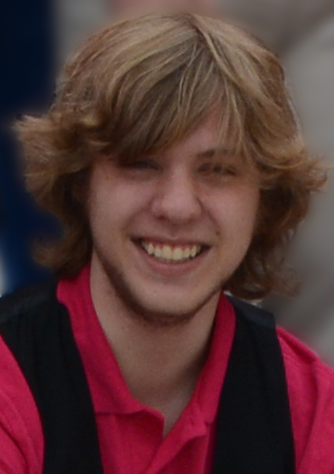
\includegraphics[width=\fibelstdlen]{res/vorstellungsfotos/jonas_kausch.png}
	\end{wrapfigure}
}
{Das ist Justus. Eigentlich heißt der Fachschafts-Doctor im 5.~Semester Jonas.
Prinzipiell ist er immer für eine ausgiebige Diskussion zu haben, sei es zu "Doctor Who", den Feinheiten der Kampfsysteme des antiken Griechenlands oder einem beliebigen anderen Thema, mit dem er sich selbstverständlich auskennt.
Allerdings ist er nicht immer besonders zuverlässig -- deswegen berichtet er hier nicht selbst über sich ;-)}

% \begin{center}
% 	
\includegraphics[width=\columnwidth]{res/fsphys_logo.pdf}
% \end{center}

\fibelvorstellung{
	\begin{wrapfigure}{r}{0cm}
		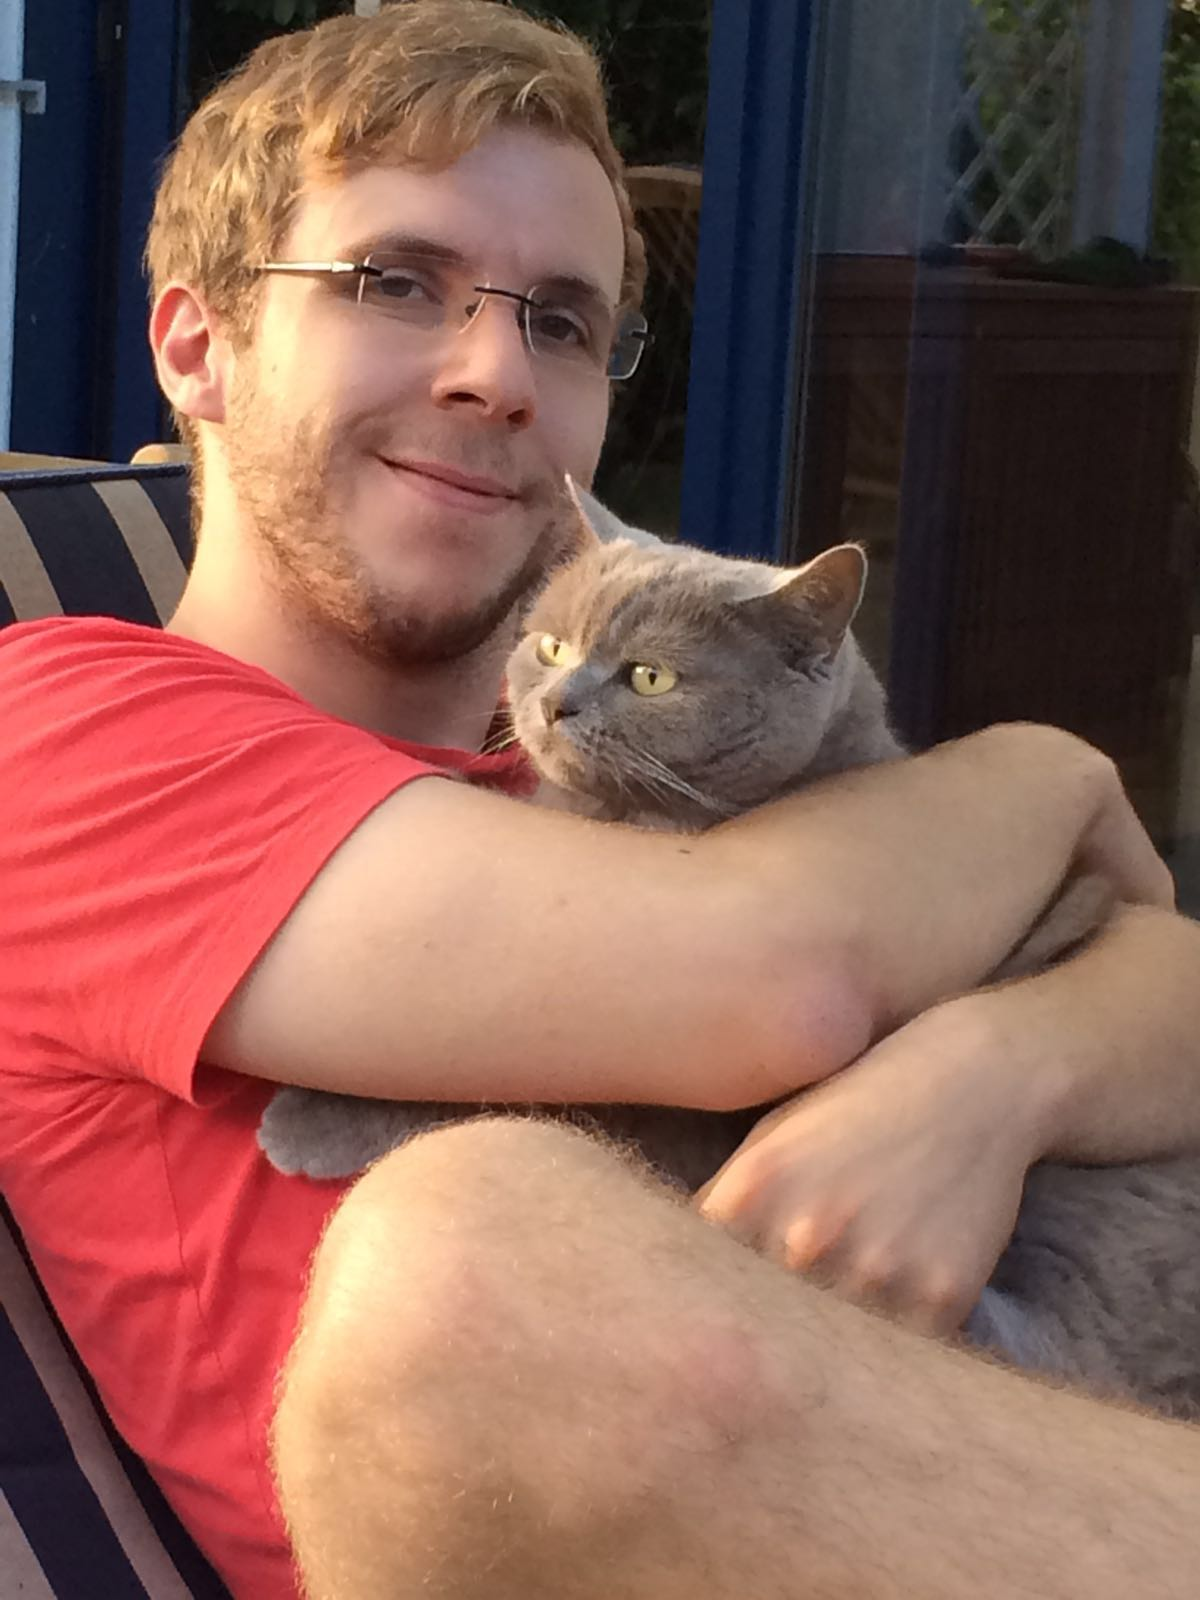
\includegraphics[width=\fibelstdlen]{res/vorstellungsfotos/lukas_eschmann.jpg}
	\end{wrapfigure}
}
{moin, ich bin Lukas und in den letzten Zügen meines Studiums. Ich war
vom ersten bis zum letzten Semester in der Fachschaft und werde mich
auch noch in meiner Promotion weiter hier engagieren.
In meiner Zeit hier hatte ich schon verschiedene Aufgaben, setze mich
aber vor allem in den Hochschulgremien am Fachbereich für euch ein!
Privat geh ich viel tanzen und sitze auch gerne noch lange nach der
Fachschaftssitzung mit den anderen Fachschaftlern auf ein zwei Bierchen
in der Fachschaft. Wenn ihr Lust habt, schaut doch auch mal vorbei. Wie
immer freue ich mich auch dieses Jahr ganz besonders auf eure O-Woche,
euer Ersti-Wochenende und natürlich auch auf euch.}

\fibelvorstellung{
	\begin{wrapfigure}{l}{0cm}
		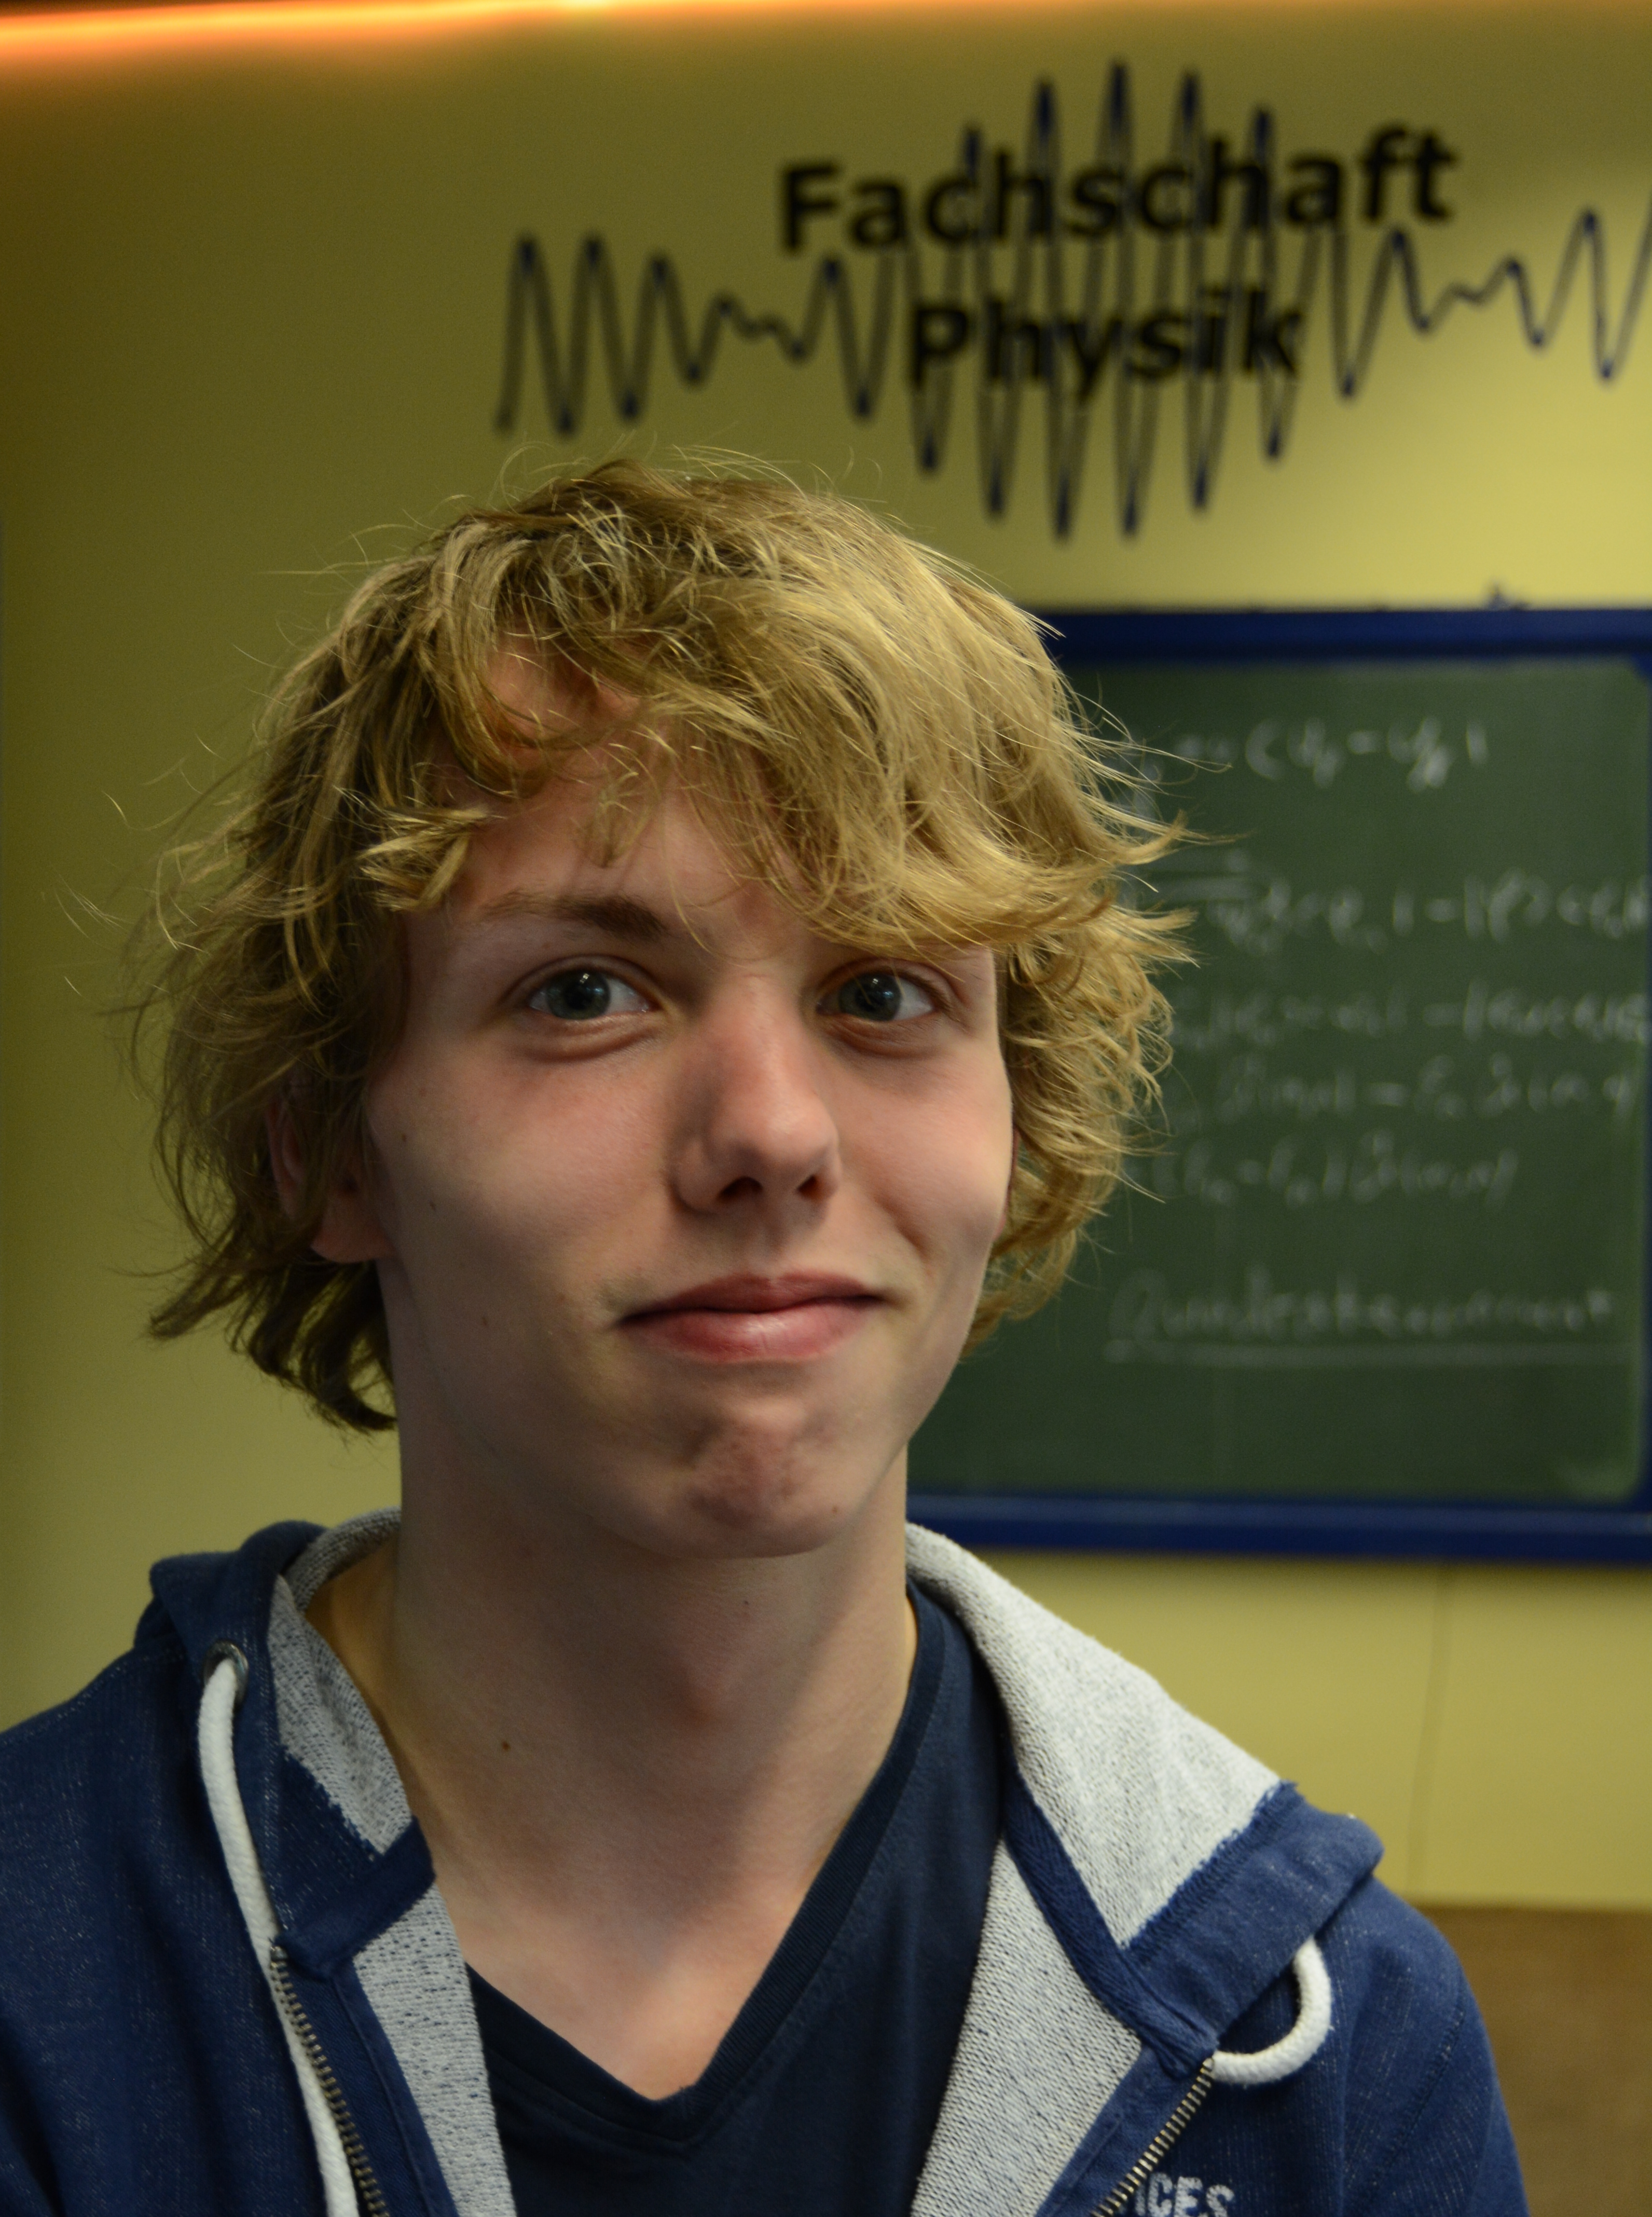
\includegraphics[width=\fibelstdlen]{res/vorstellungsfotos/marius_willer_cropped.jpg}
	\end{wrapfigure}
}
{Hi, ich bin Marius und heiße euch ebenfalls hier an der Uni Münster im Fachbereich Physik willkommen. 
Auch ich habe die Ersti-Woche sehr genossen und die Ersti--Fahrt/das Ersti-Wochenende war auch unbeschreiblich cool.
Ich hoffe, ihr werdet euren "Spaß" hier haben.}

\fibelvorstellung{
	\begin{wrapfigure}{r}{0cm}
		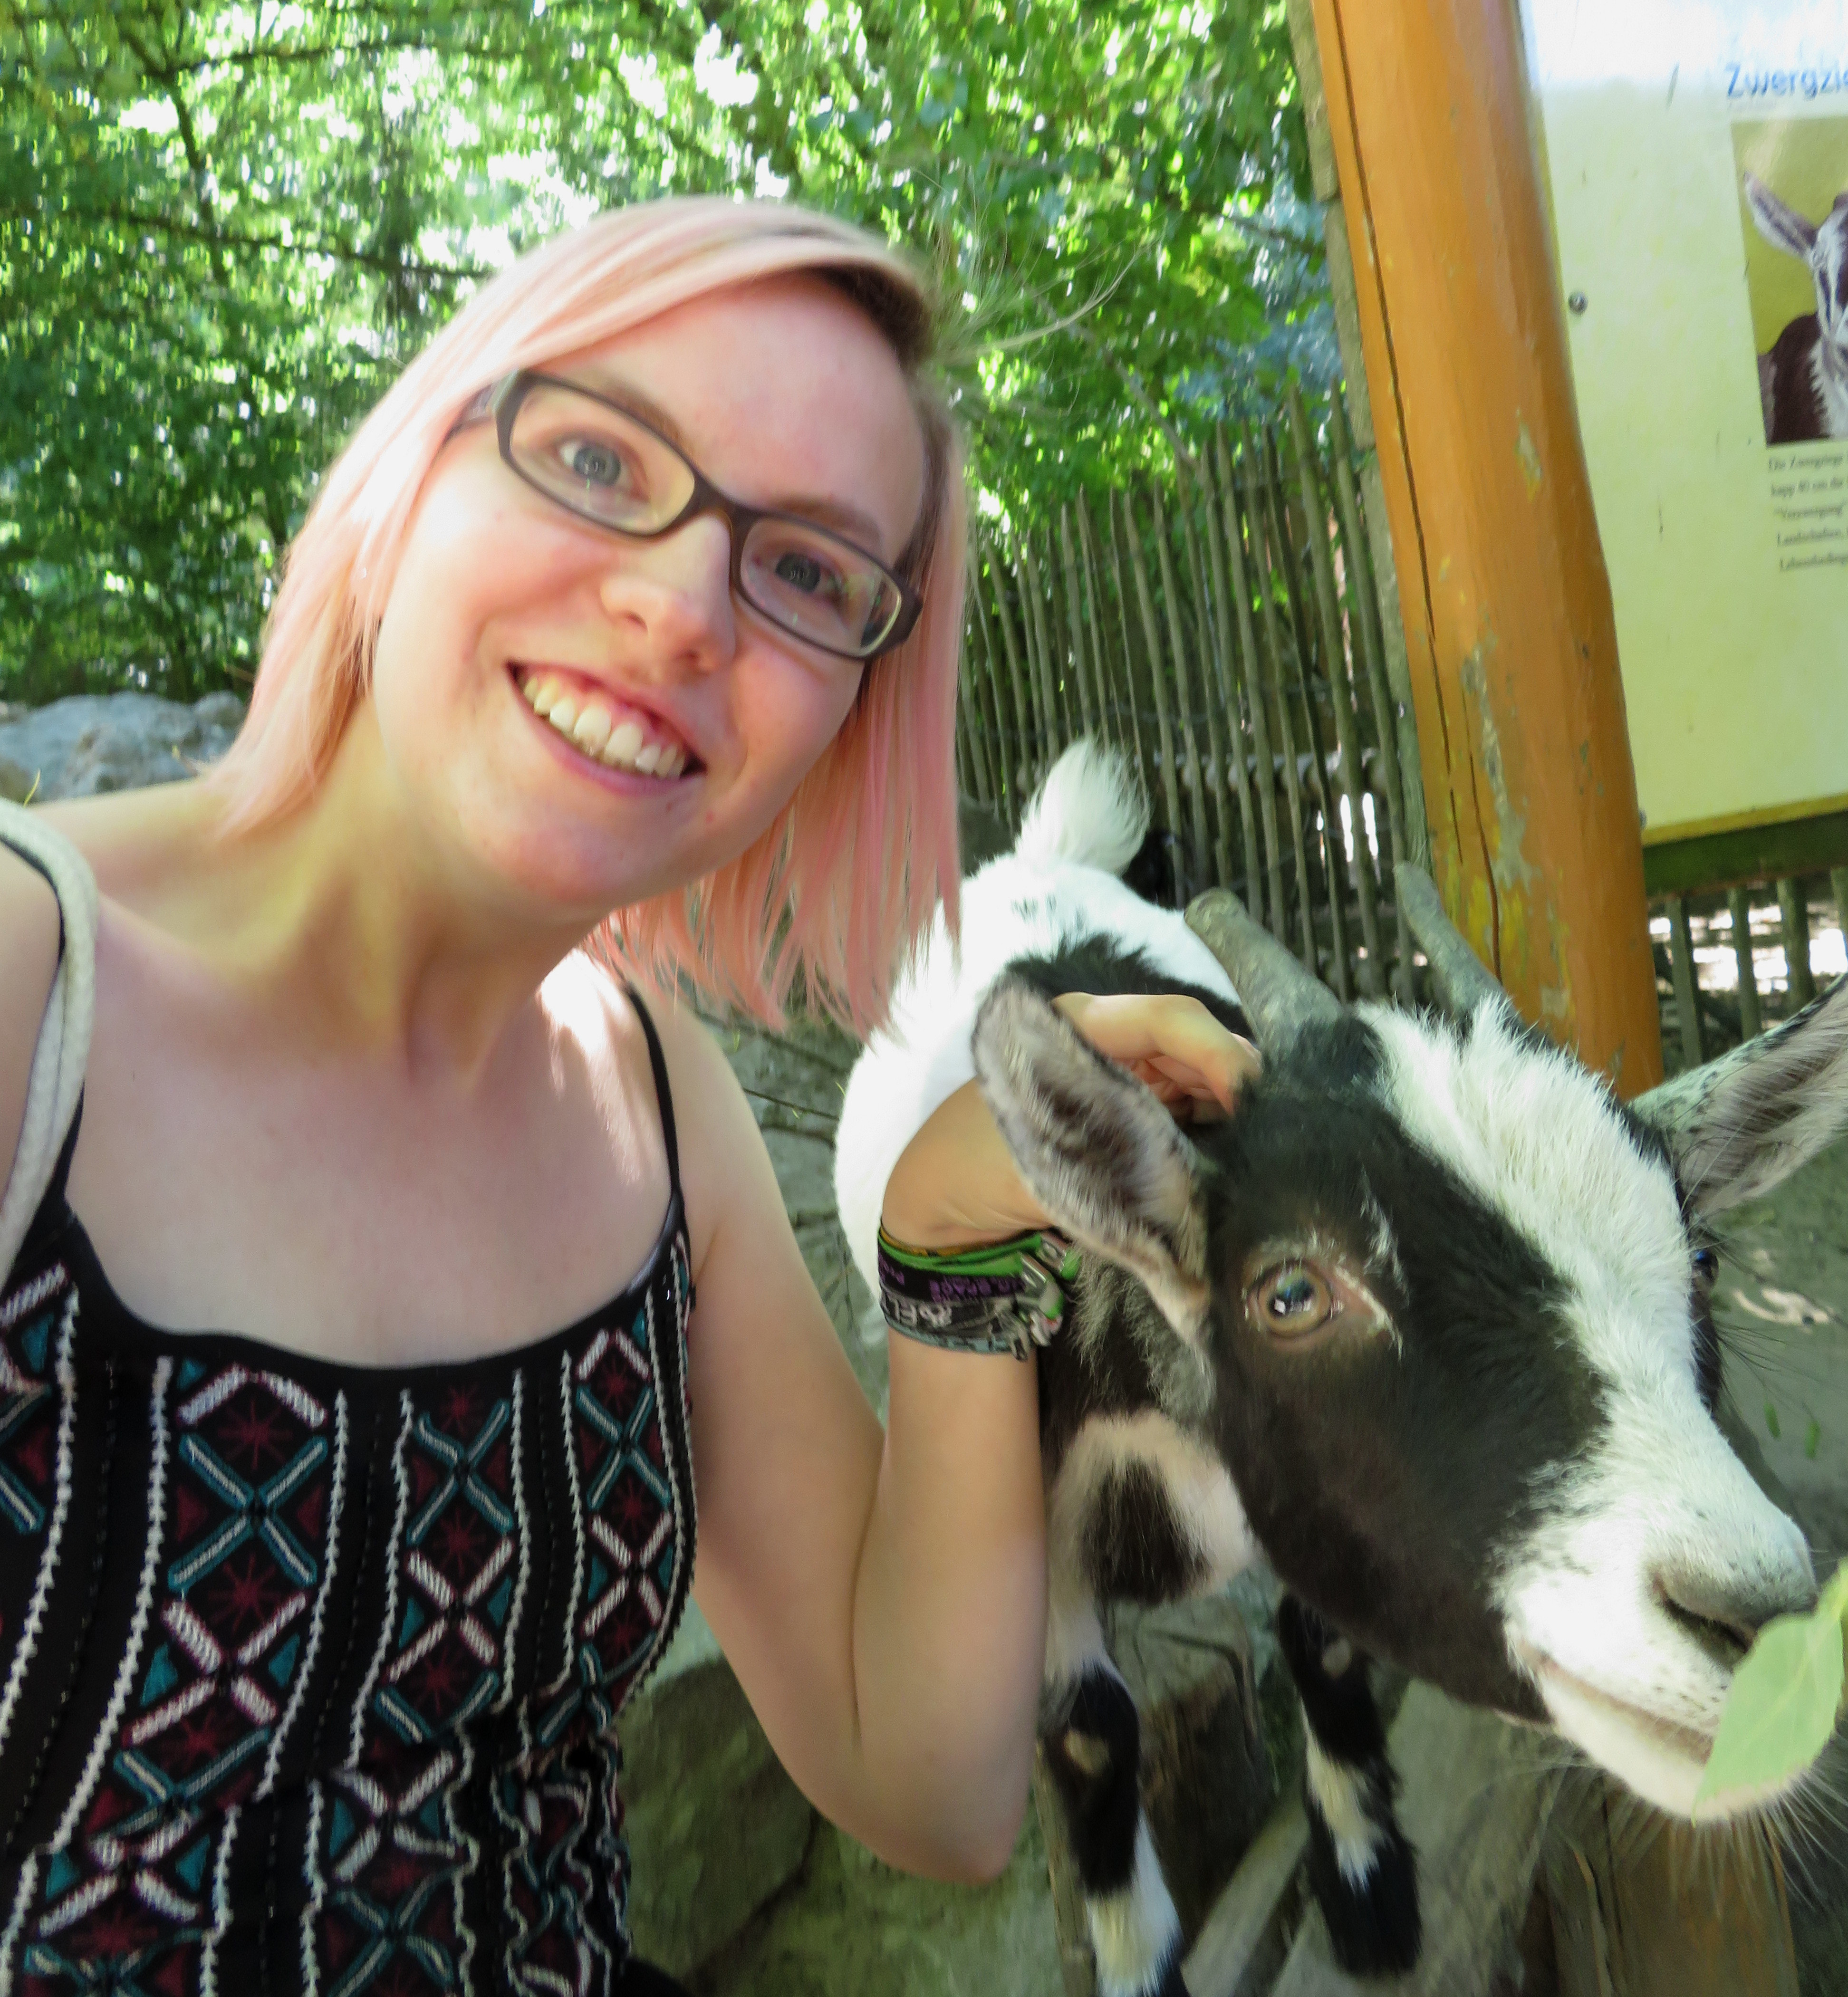
\includegraphics[width=\fibelstdlen]{res/vorstellungsfotos/miriam_neumann_cropped.jpg}
	\end{wrapfigure}
}
{Hey, ich bin Miri und fange gerade mit meinem Master an. Bei einem Tee (oder auch einem Bier ;)) könnt ihr mich gerne über das Studium oder die Stadt ausfragen. Auch falls ihr sonst etwas wissen wollt, ihr Hilfe braucht oder einfach nur quatschen wollt, seid ihr willkommen!

\vspace{1ex}}

\fibelvorstellung{
	\begin{wrapfigure}{l}{0cm}
		\includegraphics[width=\fibelstdlen]{res/vorstellungsfotos/philip_render_cropped.png}
	\end{wrapfigure}
}
{Hi, ich bin der Philip. Bin schon ein bisschen länger an der Uni und oft an der charakteristischen Bierpulle zu erkennen ;)

Als 2FB kann ich euch auch übrigens immer gut von den schönen Seiten des Physikstudiums berichten.
\vspace{\baselineskip}}

\fibelvorstellung{
	\begin{wrapfigure}{r}{0cm}
		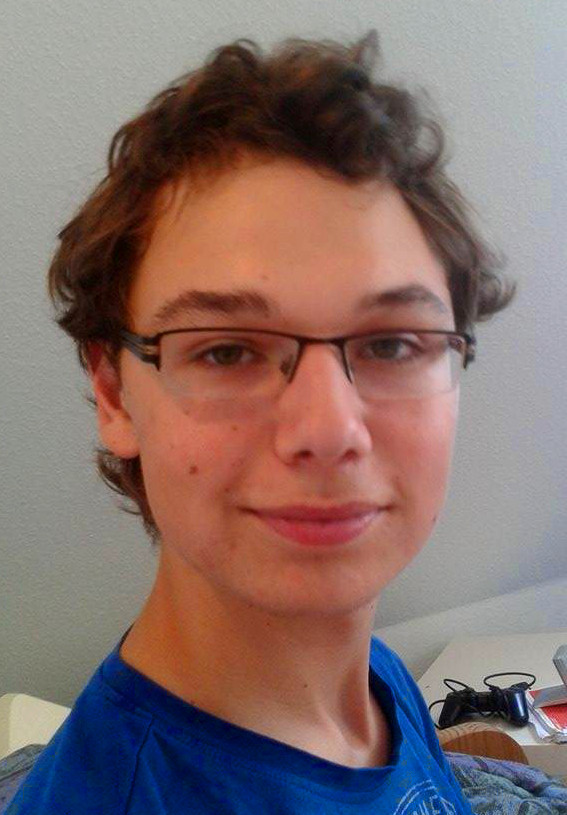
\includegraphics[width=3.2cm]{res/vorstellungsfotos/rene_henke.jpg}
	\end{wrapfigure}
}
{Ich bin der René (nicht zu verwechseln mit Rene) und studiere momentan Physik im 7.~Semester.
	Neben der Fachschaft bin ich auch in der jDPG Regionalgruppe Münster aktiv, stehe also gerne als Ansprechpartner für alles, was die jDPG betrifft, zur Seite.
	\vspace{\baselineskip}}

\fibelvorstellung{
	\begin{wrapfigure}{l}{0cm}
		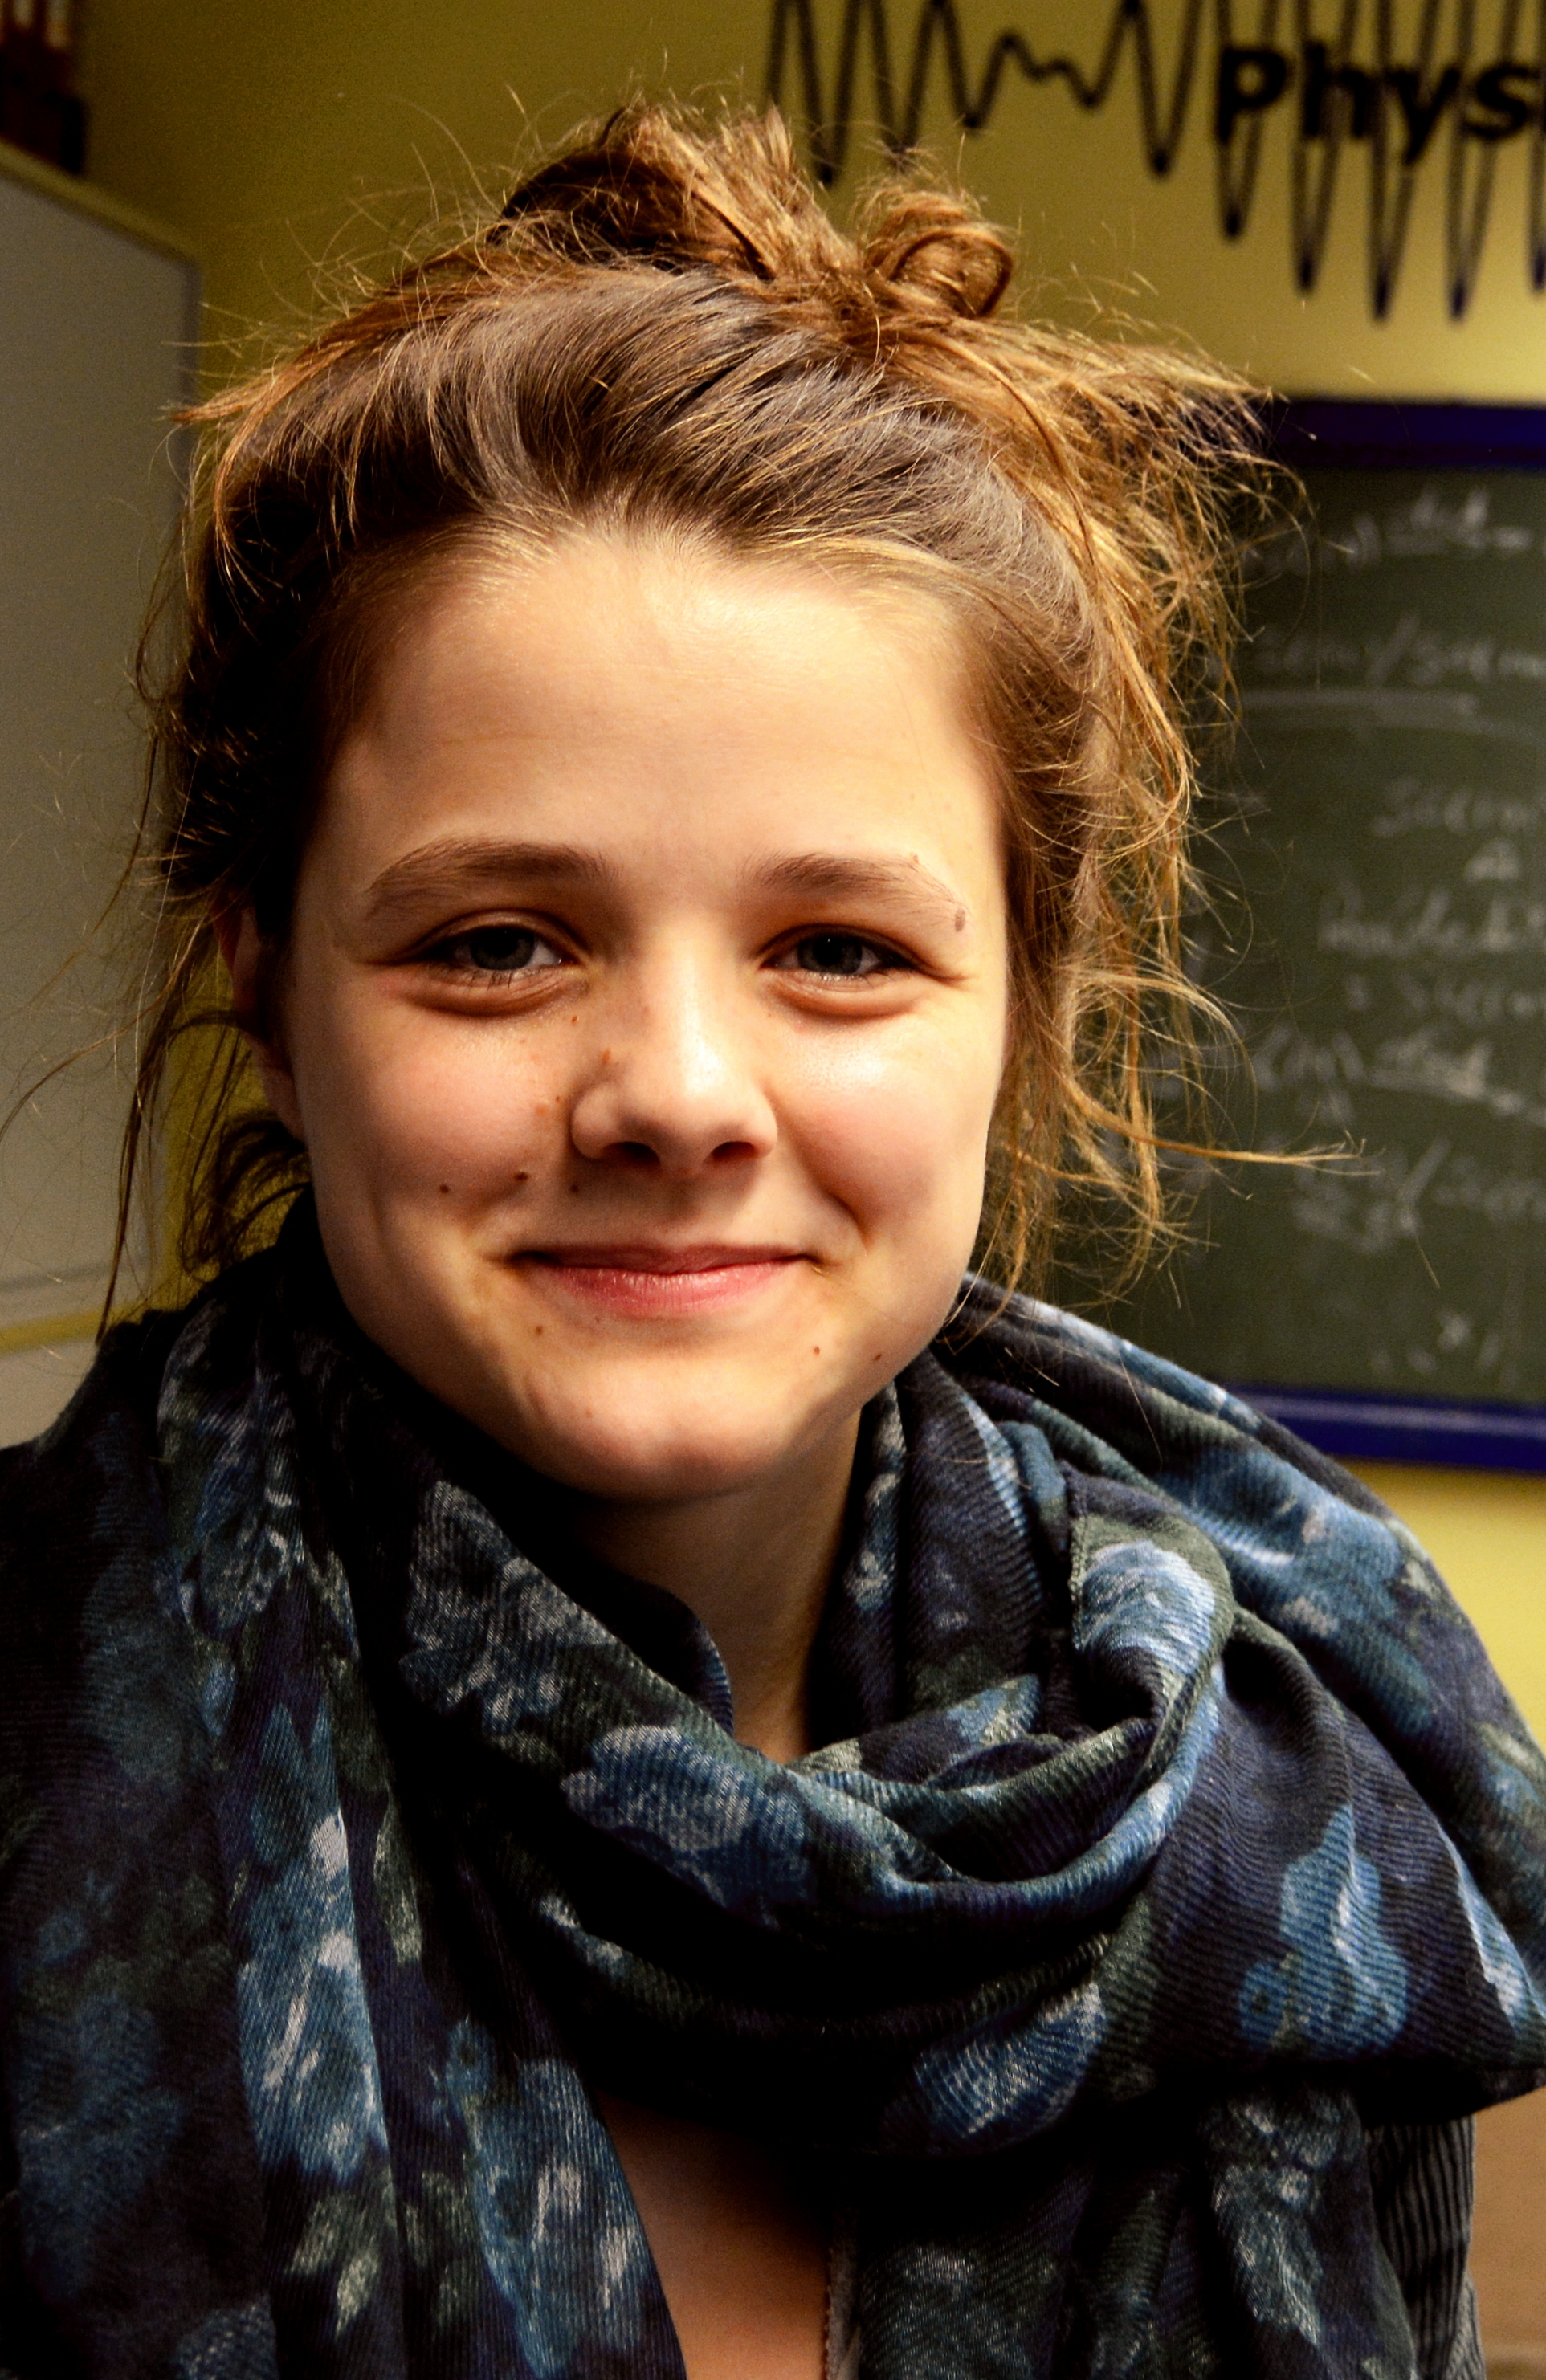
\includegraphics[width=\fibelstdlen]{res/vorstellungsfotos/pia_petrak_cropped.jpg}
	\end{wrapfigure}
}
{Hey, ich bin Pia, 20 und jetzt im 5.  Semester Physik (Ein-Fach-Bachelor). Falls ihr noch zweifelt...Physik ist wirklich cool:) 
Lasst ruhig die Sau raus in der O-Woche, wird schon früh genug ein bisschen stressiger;) Viel Spaß und hört bloß nicht auf mit Physik!:)
}

\vspace{6ex}

\fibelvorstellung{
	\begin{wrapfigure}{r}{0cm}
		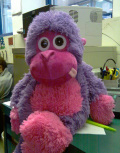
\includegraphics[width=\fibelstdlen]{res/vorstellungsfotos/fritz.png}
	\end{wrapfigure}
}
{Hallo, ich bin Fritz und bin neu in der Fachschaft Physik.
Die Mannschaft hier ist echt genial aufgestellt, sodass es richtigen Spaß macht, ein aktiver Teil der Universität Münster zu sein.
Ich kann dir nur empfehlen: Mach' mit und verändere die Uni!}
\end{multicols*}
